\scanpage{18}
\[
(2)\quad\left\{\begin{gathered}
\sigma_0^2=\sigma_1^2=\sigma_\infty^2=1\\
\sigma_0\sigma_1=\deleted{\unsure{l_0\rho}}\inserted{\rho l_0}\qquad
\unsure{\sigma_1|\dot\sigma_1}\sigma_\infty=\deleted{\unsure{l_1\rho}}\inserted{\rho l_1}\qquad
\sigma_\infty\sigma_0=\deleted{l_\infty\rho}\inserted{\rho l_\infty}
\end{gathered}\right.
\]
\margin{NB Since $\sigma_1=\rho\sigma_0\rho^{-1}\ldots$, these $\leftarrow$ relations can also be written
\[
\begin{aligned}
\deleted{\displaystyle l_0}&\deleted{\displaystyle =(\sigma_0\rho)^2\unsure{\sigma_\infty}(\unsure{l_0\sigma_0\sigma_0\rho^{-1}|\rho\sigma_0\rho^{-1}})}\\
\deleted{\displaystyle l_1}&\deleted{\displaystyle =(\sigma_1\rho)^2\unsure{\sigma_1}\qquad}&\deleted{\displaystyle \unsure{l_0}}&\deleted{\displaystyle =\unsure{\rho^{-1}\sigma_0}}\\
\deleted{\displaystyle l_\infty}&\deleted{\displaystyle =(\sigma_\infty\rho)^2\unsure{\sigma_\infty}}
\end{aligned}
\]
\begin{tabular}{|l}
$\begin{aligned}
l_0&=\rho^{-1}\sigma_0\rho\sigma_0\rho^{-1}\\
\text{\deleted{We have}}&=\rho^{-1}[\sigma_0,\rho]
\end{aligned}$\\
We have\\
$\begin{aligned}
\deleted{\sigma_0(l_0)=l_1}\\
\deleted{\sigma_0(l_1)=\unsure{l_\infty|l_0}}\\
\deleted{\sigma_0(l_\infty)=\unsure{l_1^{-1}l_0^{-1}}}
\end{aligned}$\\
$\begin{aligned}
\sigma_0(l_0)&=l_\infty^{-1}l_1^{-1}\\
\sigma_0(l_1)&=l_\infty
\end{aligned}$
\end{tabular}
\[
\sigma_0(l_\infty)=l_1
\]}
where $\rho$, over $\dot\rho$, is defined by the trivial path from $P$ \unsure{to|:} $P$. We therefore have
\[
\left\{\begin{aligned}
\rho\sigma_0\rho^{-1}&=\sigma_1\\
\rho\sigma_1\rho^{-1}&=\sigma_\infty\\
\rho\sigma_\infty\rho^{-1}&=\sigma_0
\end{aligned}\right.
\qquad\text{i.e}\quad
\left\{\begin{aligned}
\rho\sigma_0&=\sigma_1\rho\\
\rho\sigma_1&=\sigma_\infty\rho\\
\rho\sigma_\infty&=\sigma_0\rho
\end{aligned}\right.
\]
We do not see an expression for $\rho$ in terms of $\sigma_0,\sigma_1,\sigma_\infty$ alone appear --- \deleted{we see on the other hand (using the fact that $l_0,l_1,l_\infty$ with \mbox{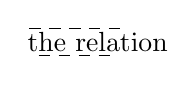
\begin{tikzpicture}[baseline=(relation.base)]
\node[inner sep=0pt,outer sep=0pt] (relation) {the relation};
\draw ([xshift=0.05em,yshift=0.35ex]relation.north west) -- ++(0.42em,0);
\draw ([xshift=0.77em,yshift=0.35ex]relation.north west) -- ++(0.42em,0);
\draw ([xshift=1.49em,yshift=0.35ex]relation.north west) -- ++(0.42em,0);
\draw ([xshift=2.21em,yshift=0.35ex]relation.north west) -- ++(0.42em,0);
\draw ([xshift=2.93em,yshift=0.35ex]relation.north west) -- ++(0.42em,0);
\draw ([xshift=0.40em,yshift=-0.35ex]relation.south west) -- ++(0.42em,0);
\draw ([xshift=1.12em,yshift=-0.35ex]relation.south west) -- ++(0.42em,0);
\draw ([xshift=1.84em,yshift=-0.35ex]relation.south west) -- ++(0.42em,0);
\draw ([xshift=2.56em,yshift=-0.35ex]relation.south west) -- ++(0.42em,0);
\end{tikzpicture}} fundamental (1) is a presentation of $\unsure{\Pi|\pi}$, that \deleted{$\rho$} \inserted{$(\sigma_0\sigma_1)^3$ (for example)} must be expressed in terms of the $l_i$; \unsure{since} in addition}
\[
\deleted{\displaystyle\deleted{\rho=l_0l_1l_\infty}}
\]
\deleted{to the \unsure{relations|relations} $\sigma_i^2=1$}, it will be necessary that $\rho$ be a product of terms $\sigma_i$ \uline{no two consecutive} \deleted{\unsure{distinct|abstract\textsuperscript{ly}}}, \deleted{\unsure{or|now} $\sigma_0\sigma_1\sigma_0=$} \inserted{and $\sigma$}
\[
\left\{\begin{aligned}
\dot\sigma_1^2=\dot\sigma_{\unsure{1|0}}^2=\dot\sigma_\infty^2&=1\\
\dot\sigma_0\dot\sigma_1=\dot\sigma_1\dot\sigma_\infty=\dot\sigma_\infty\dot\sigma_0&=\dot\rho\\
\dot\rho^3&=1
\end{aligned}\right.
\quad\text{is a presentation of }\unsure{\mathfrak S_3|\mathcal S_3}\text{\unsure{),|,}}
\]
\margin{\begin{tabular}{l}
\unsure{As we see}\\
\unsure{they|be} \unsure{of them|one} \unsure{are|of the}\\
\unsure{\uline{not} conjug\uline{ate}|\uline{not} conjugate|\uline{not} requir\uline{ed}}
\end{tabular}}
that the system of relations (1)(2) and \unsure{besides|finally|between}
\[
\rho^3=1
\]
is a presentation of the inverse image of $\unsure{\mathfrak S_3|\mathcal S_3}$ in $\mathcal E$ (say in $\widehat{\mathcal E}$, from the profinite point of view).
\margin{This is false, As we see by setting in these relations $\rho=1$, we \unsure{have} \unsure{not|no longer|then} $\unsure{\rho\sigma_0\rho^{-1}=\sigma_1}$ (?)}
\mspage{17}
